% Presentación: comparación de las pruebas unitarias de la kata Tres en Raya.
% Compilar desde esta carpeta con:  latexmk -pdf presentacion.tex
% Las cifras se leen de ../resultados/, generado por tools/compare_suites.py.

\documentclass[aspectratio=169,10pt]{beamer}

\usetheme[progressbar=frametitle,numbering=fraction,block=fill]{metropolis}

\usepackage[T1]{fontenc}
\usepackage[sfdefault,lining]{FiraSans}
\usepackage[scaled=0.82]{FiraMono}
\usepackage[spanish,es-noshorthands,es-tabla]{babel}
\usepackage{booktabs}
\usepackage{tabularx}
\usepackage{array}
\usepackage{pifont}
\usepackage{listings}
\usepackage{tikz}
\usepackage{pgfplots}
\pgfplotsset{compat=1.18}
\pgfkeys{/pgf/number format/.cd,use comma,1000 sep={}}
\usetikzlibrary{positioning,arrows.meta,shapes.misc}

% ---------------------------------------------------------------- Colores
\definecolor{colorX}{HTML}{E5484D}
\definecolor{colorO}{HTML}{1F8DC2}
\definecolor{tinta}{HTML}{23373B}
\definecolor{fondoCodigo}{HTML}{F6F4F0}
\definecolor{ok}{HTML}{2E8B57}
\definecolor{mal}{HTML}{C62828}
\definecolor{aviso}{HTML}{B25000}
\setbeamercolor{alerted text}{fg=colorX}
\setbeamercolor{block title}{bg=tinta!12,fg=tinta}
\setbeamercolor{block body}{bg=tinta!5}

% ---------------------------------------------------------------- Métricas generadas
% Archivo generado por tools/compare_suites.py: no editar a mano.
\expandafter\def\csname metric@total@mutants\endcsname{16}
\expandafter\def\csname metric@repositorio@cases\endcsname{85}
\expandafter\def\csname metric@repositorio@failures\endcsname{0}
\expandafter\def\csname metric@repositorio@assertions\endcsname{165}
\expandafter\def\csname metric@repositorio@testlines\endcsname{699}
\expandafter\def\csname metric@repositorio@lines\endcsname{100.0}
\expandafter\def\csname metric@repositorio@branches\endcsname{100.0}
\expandafter\def\csname metric@repositorio@regions\endcsname{100.0}
\expandafter\def\csname metric@repositorio@killed\endcsname{16}
\expandafter\def\csname metric@repositorio@score\endcsname{100}
\expandafter\def\csname metric@repositorio@linestext\endcsname{100,0}
\expandafter\def\csname metric@repositorio@perCase\endcsname{1,9}
\expandafter\def\csname metric@iabasico@cases\endcsname{11}
\expandafter\def\csname metric@iabasico@failures\endcsname{0}
\expandafter\def\csname metric@iabasico@assertions\endcsname{11}
\expandafter\def\csname metric@iabasico@testlines\endcsname{103}
\expandafter\def\csname metric@iabasico@lines\endcsname{64.0}
\expandafter\def\csname metric@iabasico@branches\endcsname{83.3}
\expandafter\def\csname metric@iabasico@regions\endcsname{74.3}
\expandafter\def\csname metric@iabasico@killed\endcsname{5}
\expandafter\def\csname metric@iabasico@score\endcsname{31}
\expandafter\def\csname metric@iabasico@linestext\endcsname{64,0}
\expandafter\def\csname metric@iabasico@perCase\endcsname{1,0}
\expandafter\def\csname metric@iaestructurado@cases\endcsname{23}
\expandafter\def\csname metric@iaestructurado@failures\endcsname{1}
\expandafter\def\csname metric@iaestructurado@assertions\endcsname{40}
\expandafter\def\csname metric@iaestructurado@testlines\endcsname{194}
\expandafter\def\csname metric@iaestructurado@lines\endcsname{96.8}
\expandafter\def\csname metric@iaestructurado@branches\endcsname{100.0}
\expandafter\def\csname metric@iaestructurado@regions\endcsname{97.1}
\expandafter\def\csname metric@iaestructurado@killed\endcsname{14}
\expandafter\def\csname metric@iaestructurado@score\endcsname{88}
\expandafter\def\csname metric@iaestructurado@linestext\endcsname{96,8}
\expandafter\def\csname metric@iaestructurado@perCase\endcsname{1,7}

\newcommand{\metric}[2]{\csname metric@#1@#2\endcsname}
\newcommand{\killed}{\textcolor{ok}{\ding{51}}}
\newcommand{\survived}{\textcolor{mal}{\ding{55}}}
\newcommand{\si}{\textcolor{ok}{\ding{51}}}
\newcommand{\no}{\textcolor{mal}{\ding{55}}}
\newcommand{\parcial}{\textcolor{aviso}{$\sim$}}
\newcommand{\repo}{\textbf{Repositorio}}
\newcommand{\iab}{\textbf{IA básica}}
\newcommand{\iae}{\textbf{IA estructurada}}

% ---------------------------------------------------------------- Código
\lstdefinestyle{cpp}{
  language=C++,
  basicstyle=\ttfamily\scriptsize,
  keywordstyle=\color{colorO}\bfseries,
  commentstyle=\color{gray}\itshape,
  stringstyle=\color{colorX},
  backgroundcolor=\color{fondoCodigo},
  frame=single,
  rulecolor=\color{tinta!20},
  framesep=3pt,
  xleftmargin=4pt,
  xrightmargin=4pt,
  columns=fullflexible,
  keepspaces=true,
  breaklines=true,
  showstringspaces=false,
  morekeywords={QCOMPARE,QVERIFY,QVERIFY2,QVERIFY_THROWS_EXCEPTION,QFAIL,QFETCH,constexpr,nullptr,static_assert},
  literate={á}{{\'a}}1 {é}{{\'e}}1 {í}{{\'i}}1 {ó}{{\'o}}1 {ú}{{\'u}}1
           {Á}{{\'A}}1 {É}{{\'E}}1 {Í}{{\'I}}1 {Ó}{{\'O}}1 {Ú}{{\'U}}1
           {ñ}{{\~n}}1 {Ñ}{{\~N}}1 {¿}{{?`}}1 {¡}{{!`}}1
}
\lstdefinestyle{prompt}{
  basicstyle=\ttfamily\scriptsize,
  backgroundcolor=\color{fondoCodigo},
  frame=single,
  rulecolor=\color{tinta!20},
  framesep=3pt,
  columns=fullflexible,
  keepspaces=true,
  breaklines=true,
  literate={á}{{\'a}}1 {é}{{\'e}}1 {í}{{\'i}}1 {ó}{{\'o}}1 {ú}{{\'u}}1
           {Á}{{\'A}}1 {É}{{\'E}}1 {Í}{{\'I}}1 {Ó}{{\'O}}1 {Ú}{{\'U}}1
           {ñ}{{\~n}}1 {Ñ}{{\~N}}1 {¿}{{?`}}1 {¡}{{!`}}1
}
\lstset{style=cpp}

% Capa del diagrama de arquitectura (los estilos con parámetros van fuera de los frames)
\tikzset{capa/.style={draw=tinta!60,fill=#1,rounded corners=3pt,minimum width=6.4cm,
                      minimum height=1.05cm,align=center,font=\footnotesize}}

% Tablero de 3x3 dibujado con TikZ:
%   \tablero{posiciones de X}{posiciones de O}{dibujo bajo las piezas}
% Cada posición es columna/fila, de 1 a 3, con la fila 1 arriba.
\newcommand{\tablero}[3]{%
  \begin{tikzpicture}[scale=0.55]
    #3
    \draw[tinta!50,line width=0.8pt] (1,0) -- (1,3) (2,0) -- (2,3) (0,1) -- (3,1) (0,2) -- (3,2);
    \foreach \c/\r in {#1} \node[text=colorX,font=\bfseries\large] at (\c-0.5,3.5-\r) {X};
    \foreach \c/\r in {#2} \node[text=colorO,font=\bfseries\large] at (\c-0.5,3.5-\r) {O};
  \end{tikzpicture}}

% ---------------------------------------------------------------- Portada
\title{Pruebas unitarias para la kata Tres en Raya}
\subtitle{Suite del repositorio (TDD) frente a pruebas generadas por IA}
\author{Franco Parra}
\institute{Gestión de Calidad de Sistemas · Universidad Católica Boliviana «San Pablo»}
\date{Octubre de 2026}

\begin{document}

\maketitle

\begin{frame}{Contenido}
  \setbeamertemplate{section in toc}[sections numbered]
  \tableofcontents
\end{frame}

% ======================================================================== Contexto
\section{Contexto}

\begin{frame}{La kata del Tres en Raya}
  \begin{columns}[T,onlytextwidth]
    \column{0.32\textwidth}
    \begin{block}{R1 · Tablero de 3x3}
      \footnotesize
      \begin{itemize}
        \item Fuera del eje X $\Rightarrow$ excepción
        \item Fuera del eje Y $\Rightarrow$ excepción
        \item Casilla ocupada $\Rightarrow$ excepción
      \end{itemize}
    \end{block}
    \column{0.32\textwidth}
    \begin{block}{R2 · Turnos}
      \footnotesize
      \begin{itemize}
        \item El primer turno es de \textcolor{colorX}{\textbf{X}}
        \item Después de X juega \textcolor{colorO}{\textbf{O}}
        \item Después de O juega X
      \end{itemize}
    \end{block}
    \column{0.32\textwidth}
    \begin{block}{R3 · Ganador}
      \footnotesize
      \begin{itemize}
        \item Sin línea completa no hay ganador
        \item Gana con una línea horizontal
        \item Gana con una línea vertical
        \item Gana con una diagonal
      \end{itemize}
    \end{block}
  \end{columns}
  \vfill
  \small Diez pruebas definidas por la kata. El objetivo del trabajo es comparar cómo las
  cubren una suite escrita con TDD y dos suites generadas por una IA a partir de un prompt.
\end{frame}

\begin{frame}{Entregables}
  \begin{columns}[c,onlytextwidth]
    \column{0.58\textwidth}
    \begin{itemize}
      \item \textbf{Repositorio público:}\\
        \href{https://github.com/SkyWing3/tres-en-raya}{\texttt{github.com/SkyWing3/tres-en-raya}}
      \item \textbf{Prompts:} \texttt{ia/prompts.md}
      \item \textbf{Respuestas de la IA, sin cambios:} \texttt{ia/respuestas/}
      \item \textbf{Mediciones reproducibles:} \texttt{tools/compare\_suites.py}\\
        $\rightarrow$ \texttt{docs/resultados/}
      \item \textbf{Esta presentación:} \texttt{docs/presentacion/}
      \item \textbf{Integración continua:} GitHub Actions en Linux, macOS y Windows
    \end{itemize}
    \column{0.38\textwidth}
    \centering
    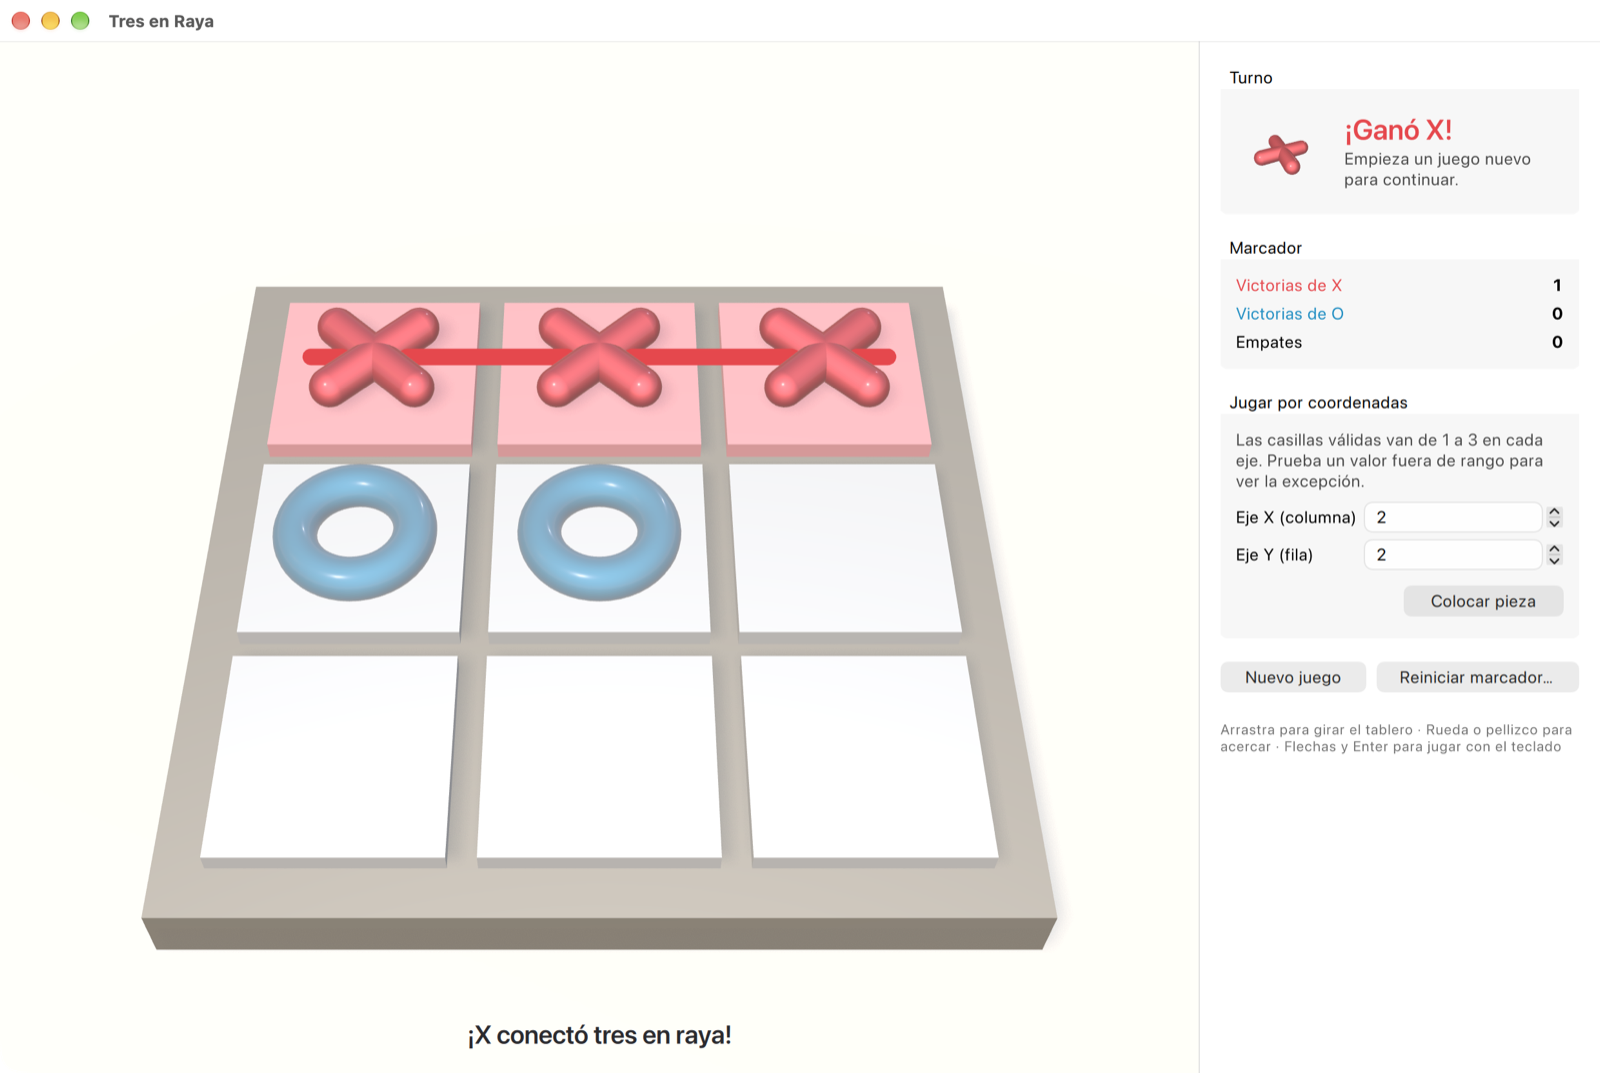
\includegraphics[width=\linewidth]{../victoria-modo-claro.png}\\[2pt]
    {\scriptsize Aplicación Qt con tablero en 3D}
  \end{columns}
\end{frame}

\begin{frame}{La solución: dominio separado de la interfaz}
  \begin{columns}[c,onlytextwidth]
    \column{0.55\textwidth}
    \begin{tikzpicture}[flecha/.style={-{Latex[length=2mm]},thick,tinta!60}]
      \node[capa=colorO!12] (app) {\textbf{Vista} (QML + Qt Quick 3D)\\controles nativos de macOS y Windows};
      \node[capa=tinta!8,below=0.45cm of app] (vm) {\textbf{ViewModel} (\texttt{GameController}, \texttt{BoardModel})\\convierte excepciones en mensajes};
      \node[capa=colorX!12,below=0.45cm of vm] (core) {\textbf{Dominio} en C++20 puro, sin Qt\\\texttt{Board}, \texttt{TicTacToe}, excepciones};
      \draw[flecha] (app) -- (vm);
      \draw[flecha] (vm) -- (core);
    \end{tikzpicture}
    \column{0.42\textwidth}
    \small
    \begin{itemize}
      \item Las reglas de la kata viven en el dominio y se prueban \alert{sin interfaz}.
      \item Excepciones con datos: \texttt{OutOfBoardException} informa el eje y el valor.
      \item Una jugada inválida no modifica la partida.
      \item Qt Test, CMake con presets y advertencias como errores (\texttt{-Werror}).
    \end{itemize}
  \end{columns}
\end{frame}

% ======================================================================== Metodología
\section{Metodología}

\begin{frame}{Tres suites de pruebas}
  \footnotesize
  \begin{tabularx}{\textwidth}{>{\raggedright\arraybackslash}p{2.6cm}X>{\raggedright\arraybackslash}p{4.2cm}}
    \toprule
    \textbf{Suite} & \textbf{Cómo se obtuvo} & \textbf{Ubicación} \\
    \midrule
    \repo{} (TDD) & Escrita con TDD junto con el código, compilando y ejecutando en cada paso, con asistencia de Claude Code. Incluye el ViewModel. & \texttt{tests/tictactoe/}\newline\texttt{tests/presentation/} \\
    \midrule
    \iab{} & Respuesta de la IA al prompt 1: sólo los requerimientos de la kata, sin el código. & \texttt{tests/ia/basico/} \\
    \midrule
    \iae{} & Respuesta de la IA al prompt 2: rol, contexto técnico, API real y reglas de calidad. & \texttt{tests/ia/estructurado/} \\
    \bottomrule
  \end{tabularx}
  \vfill
  \begin{itemize}
    \item Las suites de IA se generaron con \textbf{Claude} (Anthropic) en \alert{una sola respuesta} y se
      compilaron \alert{sin modificarlas}, con las mismas advertencias estrictas.
    \item La suite básica supuso su propia API: se ejecutó mediante un \textbf{adaptador} de unas 30 líneas
      escrito por el equipo.
  \end{itemize}
\end{frame}

\begin{frame}[fragile]{Prompt 1: básico}
  \begin{columns}[T,onlytextwidth]
    \column{0.62\textwidth}
\begin{lstlisting}[style=prompt]
Genera las pruebas unitarias en C++ usando Qt Test para la
siguiente kata de TDD de Tres en Raya:

Requerimiento 1: Una pieza puede estar colocada en un espacio
de un tablero 3x3
Pruebas:
- Cuando una pieza está fuera del eje X, entonces se debe
  lanzar una excepción
- ...
Requerimiento 2: Debe existir una forma de determinar qué
jugador juega después
- ...
Requerimiento 3: Un jugador gana si es el primero en conectar
una línea de un lado a otro, o de una esquina a otra
- ...
\end{lstlisting}
    \column{0.34\textwidth}
    \small
    \textbf{Estrategia:} lo que escribiría un estudiante que copia el enunciado.
    \medskip

    \textbf{Resultado:}
    \begin{itemize}
      \item 11 pruebas, una por cada prueba de la kata
      \item Nombres \emph{given/when/then}
      \item \alert{Inventa la API}: \texttt{play()} devuelve un texto
    \end{itemize}
  \end{columns}
\end{frame}

\begin{frame}[fragile]{Prompt 2: estructurado}
  \begin{columns}[T,onlytextwidth]
    \column{0.62\textwidth}
\begin{lstlisting}[style=prompt]
Actúa como un ingeniero de software especializado en pruebas
unitarias para C++.
## Contexto
- C++20, Qt 6.10+, Qt Test, -Werror ...
- El dominio YA está implementado. Esta es su API pública:
  class TicTacToe { GameStatus play(Position); ... };
  class OutOfBoardException { Axis axis(); int value(); };
## Requerimientos de la kata ...
## Reglas para las pruebas
3. Verifica el TIPO concreto de la excepción y sus datos.
4. Usa pruebas guiadas por datos para las 3 filas, las 3
   columnas y las 2 diagonales.
5. Incluye casos límite: 0 y 4, negativos, empate, victoria
   en la última jugada, jugar después de terminar...
\end{lstlisting}
    \column{0.34\textwidth}
    \small
    \textbf{Añade:} rol, contexto técnico, la API real y reglas de calidad.
    \medskip

    \textbf{Resultado:}
    \begin{itemize}
      \item 23 casos, compila a la primera
      \item Excepciones tipadas y pruebas guiadas por datos
      \item \alert{Una prueba defectuosa}
    \end{itemize}
  \end{columns}
\end{frame}

\begin{frame}[fragile]{Cómo se midió}
  \begin{columns}[T,onlytextwidth]
    \column{0.48\textwidth}
    \begin{block}{Métricas}
      \small
      \begin{itemize}
        \item Casos ejecutados, aserciones y líneas de prueba
        \item \textbf{Cobertura} de líneas y ramas del dominio con \texttt{llvm-cov}
        \item \textbf{Puntaje de mutación}: porcentaje de errores introducidos a propósito que la suite detecta
      \end{itemize}
    \end{block}
    \small
    Todo se calcula con \texttt{tools/compare\_suites.py} sobre una copia temporal del
    proyecto. Cada prueba se ejecuta en su propio proceso.
    \column{0.48\textwidth}
    \begin{block}{Ejemplo de mutante (M3)}
\begin{lstlisting}
// Original
return coordinate >= kMinCoordinate
    && coordinate <= kMaxCoordinate;
// Mutante: ahora acepta la coordenada 4
return coordinate >= kMinCoordinate
    && coordinate <= kMaxCoordinate + 1;
\end{lstlisting}
      \small
      Si alguna prueba falla, el mutante \textcolor{ok}{\textbf{muere}} (se detectó el error).
      Si todas pasan, \textcolor{mal}{\textbf{sobrevive}}.
    \end{block}
  \end{columns}
\end{frame}

% ======================================================================== Resultados
\section{Resultados}

\begin{frame}{Resumen de las tres suites}
  \centering
  \footnotesize
  \renewcommand{\arraystretch}{1.15}
  % Archivo generado por tools/compare_suites.py: no editar a mano.
\begin{tabular}{lccc}
\toprule
Métrica & \textbf{Repositorio (TDD)} & \textbf{IA: prompt básico} & \textbf{IA: prompt estructurado} \\
\midrule
Casos ejecutados & 85 & 11 & 23 \\
Casos que fallan sin mutantes & 0 & 0 & 1 \\
Aserciones & 161 & 11 & 40 \\
Líneas de código de prueba & 695 & 103 & 194 \\
Cobertura de líneas (dominio) & 100.0\,\% & 64.0\,\% & 96.8\,\% \\
Cobertura de ramas (dominio) & 100.0\,\% & 83.3\,\% & 100.0\,\% \\
Mutantes detectados & 16 de 16 & 5 de 16 & 14 de 16 \\
Puntaje de mutación & 100\,\% & 31\,\% & 88\,\% \\
\bottomrule
\end{tabular}

  \vfill
  \raggedright
  \footnotesize Cobertura medida sobre el dominio (\texttt{src/core}). La suite del repositorio
  además prueba el ViewModel, con 99,6\,\% de líneas cubiertas en todo el proyecto.
\end{frame}

\begin{frame}{Cobertura no es lo mismo que calidad}
  \begin{columns}[c,onlytextwidth]
    \column{0.6\textwidth}
    \begin{tikzpicture}
      \begin{axis}[
          ybar, bar width=14pt, width=\linewidth, height=6.2cm,
          ymin=0, ymax=110, ylabel={\%}, ytick={0,25,50,75,100},
          symbolic x coords={Repositorio,IA básica,IA estructurada}, xtick=data,
          nodes near coords={\pgfmathprintnumber[use comma,fixed]{\pgfplotspointmeta}},
          nodes near coords style={font=\scriptsize},
          legend style={at={(0.5,-0.18)},anchor=north,legend columns=-1,font=\footnotesize,draw=none},
          tick label style={font=\footnotesize}, enlarge x limits=0.25,
          axis lines*=left, ymajorgrids, grid style={tinta!10}]
        \addplot[fill=colorO!70,draw=none] coordinates {
          (Repositorio,\metric{repositorio}{lines})
          (IA básica,\metric{iabasico}{lines})
          (IA estructurada,\metric{iaestructurado}{lines})};
        \addplot[fill=colorX!75,draw=none] coordinates {
          (Repositorio,\metric{repositorio}{score})
          (IA básica,\metric{iabasico}{score})
          (IA estructurada,\metric{iaestructurado}{score})};
        \legend{Cobertura de líneas, Puntaje de mutación}
      \end{axis}
    \end{tikzpicture}
    \column{0.37\textwidth}
    \small
    \begin{itemize}
      \item La IA estructurada cubre el \metric{iaestructurado}{linestext}\,\% de las líneas, pero deja vivos
        \alert{dos} mutantes.
      \item Ejecutar una línea no es lo mismo que verificar su resultado.
      \item El contexto en el prompt eleva el puntaje de \metric{iabasico}{score}\,\% a
        \metric{iaestructurado}{score}\,\%.
    \end{itemize}
  \end{columns}
\end{frame}

\begin{frame}{Mutantes detectados por cada suite}
  \centering
  \scriptsize
  \renewcommand{\arraystretch}{0.95}
  % Archivo generado por tools/compare_suites.py: no editar a mano.
\begin{tabular}{llp{5.6cm}ccc}
\toprule
& Req. & Error introducido & \textbf{Repo} & \textbf{IA básica} & \textbf{IA estruct.} \\
\midrule
M1 & R1 & Rechaza la coordenada 3 (límite superior excluido) & \killed & \killed & \killed \\
M2 & R1 & Acepta la coordenada 0 & \killed & \survived & \killed \\
M3 & R1 & Acepta la coordenada 4 & \killed & \survived & \killed \\
M4 & R1 & Informa el eje equivocado al salir del eje X & \killed & \survived & \killed \\
M5 & R1 & Permite jugar sobre una casilla ocupada & \killed & \killed & \killed \\
M6 & R1 & El tablero nunca se considera lleno & \killed & \survived & \killed \\
M7 & R2 & El primer turno es de O & \killed & \killed & \killed \\
M8 & R2 & Los turnos no alternan & \killed & \killed & \killed \\
M9 & R2 & Una jugada inválida consume el turno & \killed & \survived & \survived \\
M10 & R3 & No reconoce la diagonal secundaria & \killed & \killed & \killed \\
M11 & R3 & No reconoce la tercera columna & \killed & \survived & \killed \\
M12 & R3 & No reconoce la fila inferior & \killed & \survived & \killed \\
M13 & R3 & Un tablero lleno es empate aunque haya línea & \killed & \survived & \survived \\
M14 & R3 & Se puede seguir jugando después de ganar & \killed & \survived & \killed \\
M15 & R3 & winner() informa un ganador cuando nadie ganó & \killed & \survived & \killed \\
M16 & R3 & reset() no reinicia el estado de la partida & \killed & \survived & \killed \\
\bottomrule
\end{tabular}

  \par\medskip
  \killed{} detectado \qquad \survived{} sobrevive
\end{frame}

% ======================================================================== Diferencias
\section{Diferencias sustanciales}

\begin{frame}[fragile]{1. API inventada frente a API real}
  \begin{columns}[T,onlytextwidth]
    \column{0.48\textwidth}
    \textbf{IA básica}: supone una API propia
\begin{lstlisting}
class TicTacToe {
public:
    // "No hay ganador" o "X es el ganador"
    QString play(int x, int y);
    char nextPlayer() const;
};
QCOMPARE(actual, QString("X es el ganador"));
\end{lstlisting}
    \column{0.48\textwidth}
    \textbf{Repositorio}: tipos del dominio
\begin{lstlisting}
GameStatus play(Position position);
Player nextPlayer() const noexcept;
std::optional<Player> winner() const;
std::optional<Line> winningLine() const;

QCOMPARE(status, GameStatus::Won);
QCOMPARE(m_game.winningLine(),
         (Line{{{1, y}, {2, y}, {3, y}}}));
\end{lstlisting}
  \end{columns}
  \medskip
  \small
  \begin{itemize}
    \item Sin conocer el código, la IA \alert{no puede compilar} contra el proyecto: se necesitó un adaptador.
    \item Comparar textos es frágil: un cambio de redacción rompe las pruebas sin que cambie el comportamiento.
    \item El repositorio verifica también \emph{qué} línea ganó, no sólo que alguien ganó.
  \end{itemize}
\end{frame}

\begin{frame}[fragile]{2. Excepciones genéricas frente a excepciones tipadas}
  \begin{columns}[T,onlytextwidth]
    \column{0.44\textwidth}
    \textbf{IA básica}
\begin{lstlisting}
QVERIFY_THROWS_EXCEPTION(std::runtime_error,
                         ticTacToe->play(5, 2));
\end{lstlisting}
    \small
    \begin{itemize}
      \item Cualquier error pasa la prueba: fuera del eje X, del eje Y u ocupada.
      \item Mutante M4 (informa el eje equivocado): \survived
    \end{itemize}
    \column{0.52\textwidth}
    \textbf{Repositorio}
\begin{lstlisting}
try {
    m_game.play({x, 2});
    QFAIL("Se esperaba OutOfBoardException");
} catch (const OutOfBoardException &exception) {
    QCOMPARE(exception.axis(), Axis::X);
    QCOMPARE(exception.value(), x);
}
\end{lstlisting}
    \small
    \begin{itemize}
      \item Verifica el tipo exacto, el eje y el valor rechazado.
      \item Mutante M4: \killed
    \end{itemize}
  \end{columns}
\end{frame}

\begin{frame}[fragile]{3. Valores límite y pruebas guiadas por datos}
  \begin{columns}[T,onlytextwidth]
    \column{0.42\textwidth}
    \textbf{IA básica}: un solo valor, lejos del límite
\begin{lstlisting}
ticTacToe->play(5, 2);  // eje X
ticTacToe->play(2, 5);  // eje Y
\end{lstlisting}
    \small
    Si el juego aceptara el 0 o el 4 (M2, M3), las pruebas seguirían pasando: \survived
    \column{0.54\textwidth}
    \textbf{Repositorio}: \texttt{\_data()} + \texttt{QFETCH}
\begin{lstlisting}
QTest::newRow("x = 0") << 0;
QTest::newRow("x = 4") << 4;
QTest::newRow("x = -1") << -1;
QTest::newRow("x = INT_MIN")
    << std::numeric_limits<int>::min();
QTest::newRow("x = INT_MAX")
    << std::numeric_limits<int>::max();
\end{lstlisting}
    \small
    Una sola función de prueba recorre cada valor límite y los extremos de \texttt{int}.
  \end{columns}
\end{frame}

\begin{frame}{4. ¿Se prueban todas las formas de ganar?}
  \centering
  \small
  \begin{tabular}{lccc}
    \toprule
    \textbf{Líneas ganadoras probadas} & \repo & \iab & \iae \\
    \midrule
    Filas                       & 3 de 3 & 1 de 3 & 3 de 3 \\
    Columnas                    & 3 de 3 & 1 de 3 & 3 de 3 \\
    Diagonales                  & 2 de 2 & 2 de 2 & 2 de 2 \\
    Gana \textcolor{colorO}{\textbf{O}} & \si & \si & \no \\
    Verifica \emph{qué} línea ganó & \si & \no & \si \\
    \bottomrule
  \end{tabular}
  \vfill
  \raggedright
  \begin{itemize}
    \item La kata dice «\emph{una} línea horizontal»; la IA básica la tomó literalmente y probó sólo la fila
      superior. Si el juego no reconociera la fila inferior o la tercera columna (M11, M12), no lo notaría.
    \item Las pruebas guiadas por datos cubren las 8 líneas sin duplicar código.
  \end{itemize}
\end{frame}

\begin{frame}[fragile]{5. Una prueba defectuosa generada por la IA}
  \begin{columns}[T,onlytextwidth]
    \column{0.55\textwidth}
\begin{lstlisting}
void TestTicTacToeIA::winOnLastMoveIsNotDraw()
{
    // X O X
    // O O X
    // X X X  <- X completa la fila 3 en la novena jugada
    playSequence({{1, 1}, {2, 1}, {3, 1}, {1, 2},
                  {3, 2}, {2, 2}, {1, 3}, {2, 3}});
    QCOMPARE(m_game.play({3, 3}), GameStatus::Won);
\end{lstlisting}
    \small
    \begin{itemize}
      \item El dibujo del comentario no corresponde a la secuencia de jugadas.
      \item La novena jugada lanza \texttt{GameOverException} y Qt Test \alert{aborta todo el ejecutable}
        (código 134).
      \item Era la prueba que debía detectar M13, que \survived.
    \end{itemize}
    \column{0.4\textwidth}
    \centering
    \begin{tabular}{cc}
      {\scriptsize Lo que dice el comentario} & {\scriptsize Lo que se juega} \\[2pt]
      \tablero{1/1,3/1,3/2,1/3,2/3,3/3}{2/1,1/2,2/2}
        {\draw[colorX,dashed,rounded corners=2pt] (0.08,0.08) rectangle (2.92,0.92);} &
      \tablero{1/1,3/1,3/2,1/3}{2/1,1/2,2/2,2/3}
        {\fill[colorO!18,rounded corners=2pt] (1.08,0.08) rectangle (1.92,2.92);}
    \end{tabular}
    \par\medskip
    {\footnotesize En la octava jugada \textcolor{colorO}{\textbf{O}} ya completó la columna central.}
  \end{columns}
\end{frame}

\begin{frame}[fragile]{6. Una prueba que no puede fallar}
  \begin{columns}[T,onlytextwidth]
    \column{0.52\textwidth}
    \textbf{IA estructurada}
\begin{lstlisting}
m_game.play({1, 1}); // X
QVERIFY_THROWS_EXCEPTION(OccupiedCellException,
                         m_game.play({1, 1}));
QVERIFY_THROWS_EXCEPTION(OutOfBoardException,
                         m_game.play({4, 4}));
QCOMPARE(m_game.nextPlayer(), Player::O);
\end{lstlisting}
    \small
    Con el error M9 (una jugada inválida consume el turno), cada jugada inválida cambia el turno: X $\to$ O
    $\to$ X\ldots{} Dos cambios seguidos se anulan y la prueba \textbf{pasa}: \survived
    \column{0.44\textwidth}
    \textbf{Repositorio} (corregido)
\begin{lstlisting}
QVERIFY_THROWS_EXCEPTION(InvalidMoveException,
                         m_game.play({1, 1}));
QCOMPARE(m_game.nextPlayer(), Player::O);

QVERIFY_THROWS_EXCEPTION(InvalidMoveException,
                         m_game.play({0, 1}));
QCOMPARE(m_game.nextPlayer(), Player::O);
\end{lstlisting}
    \small
    El repositorio tenía la misma debilidad: el análisis de mutantes la reveló y se corrigió verificando
    después de \emph{cada} jugada.
  \end{columns}
\end{frame}

\begin{frame}{7. Casos que la kata no pide, pero el juego necesita}
  \centering
  \footnotesize
  \begin{tabular}{lccc}
    \toprule
    \textbf{Caso} & \repo & \iab & \iae \\
    \midrule
    Empate con el tablero lleno                    & \si & \no & \si \\
    Victoria en la última jugada (no es empate)    & \si & \no & \parcial{} defectuosa \\
    No se puede jugar después de terminar          & \si & \no & \si \\
    Una jugada inválida no cambia el turno         & \si & \no & \parcial{} enmascarada \\
    Reiniciar después de ganar                     & \si & \no & \no \\
    Extremos de \texttt{int} (\texttt{INT\_MIN}, \texttt{INT\_MAX}) & \si & \no & \no \\
    Pruebas del tablero (\texttt{Board}) de forma aislada & \si & \no & \no \\
    ViewModel: señales, marcador y mensajes para la vista & \si & \no & \no \\
    \bottomrule
  \end{tabular}
  \vfill
  \raggedright\small
  La IA sólo agrega casos límite cuando el prompt los nombra uno por uno. TDD los hace aparecer al
  diseñar cada comportamiento.
\end{frame}

\begin{frame}{8. Diseño y mantenibilidad de las pruebas}
  \centering
  \footnotesize
  \begin{tabularx}{\textwidth}{>{\raggedright\arraybackslash}p{3.2cm}*{3}{>{\raggedright\arraybackslash}X}}
    \toprule
    & \repo & \iab & \iae \\
    \midrule
    Organización & Un archivo por requerimiento, más \texttt{Board} y ViewModel & Un archivo & Un archivo \\
    Preparación (\emph{fixture}) & Objeto por valor y \texttt{init()} & \texttt{new}/\texttt{delete} manuales & Objeto por valor y \texttt{init()} \\
    Trazabilidad & Comentario que cita cada prueba de la kata & Agrupadas por requerimiento & Comentario que cita cada prueba \\
    Diagnóstico al fallar & \texttt{QFAIL}/\texttt{QVERIFY2} con mensaje & Sin mensajes & \texttt{QFAIL} con mensaje \\
    Verificación en compilación & \texttt{static\_assert} de jugadores y primer turno & No & No \\
    Aserciones por caso & \metric{repositorio}{perCase} & \metric{iabasico}{perCase} & \metric{iaestructurado}{perCase} \\
    \bottomrule
  \end{tabularx}
\end{frame}

\begin{frame}{Lo que la IA hizo bien}
  \begin{itemize}
    \item \textbf{Rapidez}: una suite completa y legible en segundos.
    \item \textbf{Estructura correcta}: una prueba por caso de la kata, nombres descriptivos y
      preparación independiente de cada prueba.
    \item Con el prompt estructurado:
      \begin{itemize}
        \item compiló a la primera con \texttt{-Werror} y contra la API real;
        \item usó excepciones tipadas y pruebas guiadas por datos;
        \item alcanzó \metric{iaestructurado}{linestext}\,\% de cobertura y \metric{iaestructurado}{score}\,\% de
          puntaje de mutación.
      \end{itemize}
    \item El prompt cambia el resultado más que la herramienta: \alert{la calidad depende de lo que se le pide}.
  \end{itemize}
\end{frame}

% ======================================================================== Conclusiones
\section{Conclusiones}

\begin{frame}{Integración continua}
  \begin{columns}[c,onlytextwidth]
    \column{0.55\textwidth}
    \begin{tikzpicture}[
        paso/.style={draw=tinta!50,fill=tinta!6,rounded corners=2pt,minimum width=4.6cm,
                     minimum height=0.62cm,font=\footnotesize},
        flecha/.style={-{Latex[length=1.6mm]},tinta!60}]
      \node[paso,fill=colorO!12] (p0) {\texttt{git push} a \texttt{main}};
      \node[paso,below=0.25cm of p0] (p1) {Instalar Qt 6.10 y Ninja};
      \node[paso,below=0.25cm of p1] (p2) {\texttt{cmake -{}-preset debug}};
      \node[paso,below=0.25cm of p2] (p3) {Compilar aplicación y pruebas};
      \node[paso,below=0.25cm of p3,fill=ok!15] (p4) {\texttt{ctest}: pruebas del repositorio};
      \node[paso,below=0.25cm of p4,fill=aviso!12] (p5) {\texttt{ctest -{}-preset ia} (informativo)};
      \foreach \a/\b in {p0/p1,p1/p2,p2/p3,p3/p4,p4/p5} \draw[flecha] (\a) -- (\b);
    \end{tikzpicture}
    \column{0.42\textwidth}
    \small
    \begin{itemize}
      \item GitHub Actions, como el flujo con Maven del repositorio de referencia, pero en
        \textbf{Linux, macOS y Windows}.
      \item Cada \texttt{push} y \emph{pull request} ejecuta las pruebas del repositorio; si alguna falla, el
        cambio queda marcado en rojo.
      \item Las suites de IA se ejecutan aparte: se conservan tal como se entregaron, con su prueba defectuosa.
    \end{itemize}
  \end{columns}
\end{frame}

\begin{frame}{Conclusiones}
  \begin{enumerate}
    \item Con sólo el enunciado, la IA produce pruebas que \alert{parecen completas} pero detectan
      \metric{iabasico}{killed} de \metric{total}{mutants} errores: cubren la letra de la kata, no el
      comportamiento.
    \item Con contexto y reglas, la IA se acerca mucho
      (\metric{iaestructurado}{killed}/\metric{total}{mutants}), pero entregó \alert{una prueba incorrecta}
      y otra que no podía fallar.
    \item La cobertura no basta: \metric{iaestructurado}{linestext}\,\% de líneas cubiertas con dos errores sin
      detectar. Las \textbf{pruebas de mutación} miden mejor la calidad.
    \item La diferencia de fondo es el \textbf{proceso}: escribir, ejecutar, medir y revisar cada prueba.
      Incluso así, el análisis encontró una debilidad en la suite del repositorio.
  \end{enumerate}
\end{frame}

\begin{frame}{Recomendaciones para usar IA al escribir pruebas}
  \begin{columns}[T,onlytextwidth]
    \column{0.48\textwidth}
    \begin{block}{En el prompt}
      \small
      \begin{itemize}
        \item Incluir la API real (encabezados) y el marco de pruebas.
        \item Pedir excepciones tipadas y sus datos.
        \item Nombrar los casos límite que importan.
        \item Pedir pruebas guiadas por datos.
      \end{itemize}
    \end{block}
    \column{0.48\textwidth}
    \begin{block}{Después de generar}
      \small
      \begin{itemize}
        \item Compilar y ejecutar \emph{antes} de aceptar.
        \item Revisar que cada prueba verifique lo que dice su nombre.
        \item Medir cobertura \textbf{y} puntaje de mutación.
        \item Integrarlas a CI como cualquier otro código.
      \end{itemize}
    \end{block}
  \end{columns}
\end{frame}

\begin{frame}{Declaración de uso de IA}
  \small
  \begin{itemize}
    \item El código del repositorio y su suite de pruebas se desarrollaron con TDD con la asistencia de
      \textbf{Claude Code} (Anthropic), compilando, ejecutando y revisando cada cambio.
    \item Las suites «IA básica» e «IA estructurada» se generaron con \textbf{Claude} a partir de los prompts
      de \texttt{ia/prompts.md}, en una sola respuesta y sin correcciones.
    \item Al venir del mismo modelo, la comparación aísla el efecto del \emph{proceso} (iterar y medir frente a
      una sola respuesta) más que el de la herramienta. Los prompts pueden repetirse en ChatGPT u otra IA.
    \item Todas las cifras se obtienen con herramientas reproducibles: \texttt{tools/compare\_suites.py} y
      \texttt{tools/coverage.sh}.
  \end{itemize}
\end{frame}

\begin{frame}{Referencias}
  \footnotesize
  \begin{itemize}
    \item K. Beck. \emph{Test-Driven Development: By Example}. Addison-Wesley, 2002.
    \item V. Farcic y A. Garcia. \emph{Test-Driven Java Development}. Packt, 2015 (kata del Tres en Raya).
    \item Y. Jia y M. Harman. «An Analysis and Survey of the Development of Mutation Testing».
      \emph{IEEE Transactions on Software Engineering}, 37(5), 2011.
    \item Repositorio de referencia del curso: \url{https://github.com/gpalabral/TDD}
    \item Qt Test: \url{https://doc.qt.io/qt-6/qttest-index.html}
    \item Clang Source-based Code Coverage: \url{https://clang.llvm.org/docs/SourceBasedCodeCoverage.html}
    \item Repositorio de este trabajo: \url{https://github.com/SkyWing3/tres-en-raya}
  \end{itemize}
\end{frame}

\begin{frame}[standout]
  ¡Gracias!\\[6pt]
  {\normalsize ¿Preguntas?}
\end{frame}

\end{document}
